\documentclass[journal]{IEEEtran}
\usepackage[latin1]{inputenc}
\usepackage[T1]{fontenc}
\usepackage{textcomp}
\usepackage[english]{babel}
\usepackage{amsmath}
\usepackage{bm}
\usepackage{url}
\usepackage{cite}
\usepackage{units}
\usepackage{graphicx}
\usepackage{booktabs}
\usepackage{flushend}
\usepackage[caption=false]{subfig}
\usepackage{bibunits,bm,booktabs,braket,calc,makeidx,paralist,rotating,scrpage2,subfig,pstricks,multido,pst-plot}
\usepackage{amsfonts}
\usepackage{amsmath}    
\usepackage{epsfig}
\usepackage{accents}
\usepackage{arydshln}
%--------------------------------------------------------------------------------------------------------------------------------------------
\usepackage{stfloats}\fnbelowfloat
\setcounter{topnumber}           {2}
\setcounter{bottomnumber}        {2}
\renewcommand{\floatpagefraction}{0.95}
\renewcommand{\topfraction}      {0.9}
\renewcommand{\bottomfraction}   {0.9}
\renewcommand{\textfraction}     {0.05}

\newcommand{\Int}{\int\limits_{-\infty}^{+\infty}}
\newcommand{\TDFD}{\unitlength1ex \begin{picture}(6.2,1.6)%
            \put(0.8,0.6){\circle{1.0}}%        % Symbol fuer die Fourier-
            \put(1.30,0.6){\line(1,0){3.25}}    % transformation t -- f   
            \put(5.05,0.6){\circle*{1.0}}\end{picture}}
\newcommand{\FDTD}{\unitlength1ex \begin{picture}(6.2,1.6)%
            \put(0.8,0.6){\circle*{1.0}}%       % Symbol fuer die Fourier-
            \put(1.30,0.6){\line(1,0){3.25}}    % transformation f -- t   
            \put(5.05,0.6){\circle{1.0}}\end{picture}}

\newcommand{\mathrmm}[1]{{#1}} 
\definecolor{gruen}{rgb}{.0,0.7,.2} 
%
\newcommand{\mbrown}[1]{\textcolor{brown}{#1}}   
\newcommand{\Mbf}[1]{\mbox{\boldmath$#1$}} 
%
\hyphenation{op-tical net-works semi-conduc-tor IEEEtran Karls-ruhe}
\begin{document}
\title{\LARGE High-Speed Antenna-Coupled Terahertz Thermocouple \\ Detectors and Mixers}
\author{Johannes A. Russer,~\IEEEmembership{Member,~IEEE,}
        Christian Jirauschek,~\IEEEmembership{Member,~IEEE,} Gergo P. Szakmany, Mark Schmidt,\\ Alexei O. Orlov, Gary H. Bernstein,~\IEEEmembership{Fellow,~IEEE},  Wolfgang Porod,~\IEEEmembership{Fellow,~IEEE}, \\ Paolo Lugli,~\IEEEmembership{Fellow,~IEEE}
        and~Peter Russer,~\IEEEmembership{Life~Fellow,~IEEE}
        % 
\thanks{

This paper is an expanded version from the IEEE MTT-S International Microwave Symposium, Phoenix, AZ, USA, 17-22 May 2015.

J. A. Russer, C. Jirauschek, M. Schmidt, P. Lugli, and P. Russer are with the Institute for Nanoelectronics, Technische Universit\"at M\"unchen, 80333 Munich, Germany.

G. P. Szakmany, A. O. Orlov, G. H. Bernstein, and  W. Porod are with the Center for Nano Science and Technology, University of Notre Dame, Notre Dame, IN
46556, U.S.A..

}}

\maketitle

\begin{abstract}
An antenna-coupled nanothermocouple (ACNTC) is an integrated structure consisting of a dipole nanoantenna and a nanothermocouple (NTC). ACNTCs are excellently suited as polarization-sensitive detectors and mixers for the long-wavelength far-infrared range around 30 THz. Radiation collected by the integrated nanoantenna and fed into the hot junction creates a temperature difference between the hot and cold junctions of the thermocouple, which results in  open-circuit voltage due to the Seebeck effect.  Due to the geometry-dependence of the Seebeck coefficient in nanowires, we could realize single-metal ACNTCs. The fundamentals of single-metal NTCs are discussed.  The thermal dynamics of NTCs is investigated showing that NTCs could exhibit mixer and detector intermediate frequency and low frequency cutoffs beyond 100~GHz. We provide  experimental evidence of ACNTCs.
\end{abstract}
\IEEEoverridecommandlockouts
\begin{keywords}
Terahertz detector, thermocouple, Seebeck effect, heat conduction
\end{keywords}
\IEEEpeerreviewmaketitle
%
%-----------------------------------------------------------------------------------------------------------------------------------------------------------------------
%
\section{Introduction}\label{Introduction}
%
%-----------------------------------------------------------------------------------------------------------------------------------------------------------------------
%
Thermocouples (TCs) are excellently suited as detectors for the long-wavelength far-infrared range around 30 THz. The detector operation of TCs is based on Joule heating of the TCs by the incident radiation and the Seebeck effect, i.e., the thermoelectric effect that directly converts a temperature difference to an electric voltage~\cite{mott_theory_1936,bakker_nanoscale_2012}.  The TC, like any thermodynamic device, is subject to the restrictions of Carnot's theorem stating that the efficiency $\eta$ of any heat engine operating between two heat reservoirs at absolute temperatures $T_1 < T_2$ is limited to a maximum value of $\eta_\mathrm{max} = (T_2-T_1)/T_2$~\cite{agrawal_thermoelectric_1997}. In order to enhance the efficiency of the TC, the radiation to be detected should be collimated within a small area of a nanothermocouple (NTC) so that the electron temperature at the NTC junction gains a strong increase. 

In this work we show that NTCs are extremely fast detectors with response times in the picosecond area. This property will open new areas of applications in the Terahertz frequency bands, so far accessible only in the microwave and millimeterwave bands so that the Terahertz bands will gain additional interest from system engineers so far mainly concerned with applications up into the millimeterwave region only.

Fast NTC detectors may be employed in imaging, communications and sensing applications. Currently, TCs are commonly used in applications for which fast response times are not critical, and cut-off frequencies of some kHz and below are sufficient, and they receive little consideration as elements in RF or THz engineering. However, fast NTCs have also a rather interesting potential for applications in microwave engineering. High efficiency is desirable in communications and sensing applications since it governs the sensitivity of the device.

Antenna-coupled nanothermocouples (ACNTCs) are integrated structures consisting of a dipole nanoantenna and a NTC connected to the antenna feed~\cite{szakmany_antenna_2013}. The nanoantenna collimates the IR energy incident within the effective aperture of the antenna and feeds it into the thermocouple. The dipole nanoantenna yields polarization-sensitive detection. This induces  a temperature difference between the hot junction at the nanoantenna feed  and the remote cold junction. Due to the Seebeck effect, an  open-circuit voltage arises across the antenna feed port. The hot junction of the NTC is located at the center of the dipole-antenna where the antenna current exhibits its maximum, resulting in optimum device response. 

In~\cite{szakmany_single-metal_2014}, we have shown that NTCs can also be formed by two nanowires of the same metal but different cross-sectional areas. Compared with conventional bi-metallic TCs, fabrication of such shape-engineered mono-metallic nanowire {TCs} is much easier, and mass-production of mono-metallic TCs could be accomplished by simple manufacturing technologies.

Since the NTC junction exhibits transverse dimensions of a few ten nanometers and the TC junction is metallic without depletion layer, there would be a frequency limitation due to a junction capacitance at the RF side in case of an ideal broad-band nanoantenna shape. Due to the non-perfect conductivity of the antenna and the finite antenna cross-sectional area at the feed point there will be some cutoff frequency, however somewhere in the far-infrared region. Since the Seebeck effect is conveyed by Joule heating, the TC is essentially a square-law detector. Due to the small thermal volume of the TC hot junction, the detector and mixer  time-constant is on the order of picoseconds. Therefore we can expect extremely high bandwidths in detector and mixer applications. In~\cite{szakmany_nano-antenna_2014}, we discussed the possible application of ACNTCs as detectors in far-infrared sensor  and communication systems. The dynamics of ACNTCs has been investigated in~\cite{russer_dynamics_2014,russer_nanostructured_2015,russer_antenna-coupled_2015} and it was shown there that due to its low thermal capacity, an ACNTC is an extremely fast square-law detector with cutoff frequencies up to several hundred GHz.

In this extended paper, we also provide experimental results confirming response times of ACNTC in the RF regime. In our investigations, we expand the theoretical model for the Seebeck coefficient of single-metal thermocouples and on the modeling framework for ACNTC in THz detector and mixer applications.
In Section~\ref{SeebeckTheory} we describe the properties of single-metal nanothermocouples (SMNTCs) and discuss the theoretical fundamentals of SMNTCs on the basis of the Seebeck theory and the Fuchs-Sondheimer model.  The fabrication of ACNTC is described in Section~\ref{Fabrication}. In Section \ref{ThermalConduction}, the thermal diffusion in the thermocouple is modeled and compact lumped-element equivalent-circuit models are established describing the electric and thermal behavior of ACNTCs. The pulse-response for the NTC is computed.  In Section \ref{Detector}, the detector and mixer properties of ACNTCs are investigated on the basis of the lumped element equivalent circuit models of ACNTCs.  Detection measurements with a modulated CO$_2$ laser operating at 10.6~$\mu$m are presented in Section~\ref{Measurements}.
%
%-----------------------------------------------------------------------------------------------------------------------------------------------------------------------
%
\section{Theoretical Model for the Seebeck Coefficient of a Single-Metal Thermocouple}
\label{SeebeckTheory}
%
%-----------------------------------------------------------------------------------------------------------------------------------------------------------------------
TCs composed by two
conductors $A$ and $B$ with Seebeck coefficients $S_{A}$ and $S_{B}$,
containing two junctions show an open-circuit Seebeck voltage $v_{S}$
\begin{equation}\label{SVoltage}
v_{S}=\Delta T(S_{A}-S_{B})\,,
\end{equation}
if there is a temperature difference $\Delta T$ between the two junctions.
Usually thermocouples are made from two different metals exhibiting different
Seebeck coefficients. Demodara et al.~\cite{damodara_size_1987} have shown that in thin films the
reduction of the electron mean free path by additional scattering yields a
thickness dependence of the Seebeck coefficients.
The calculation of this geometry-dependent Seebeck coefficient is essential in
order to determine the efficiency of single metal thermocouples, as used for
detecting radiation in the terahertz regime from a nanoantenna
\cite{szakmany_antenna_2013}. As compared to thin films, thin wires which are used for the NTCs only have two
additional surface scattering planes, thus the size effect can be expected to be a scaled problem. Calculations for the conductivity of a thin wire were done by Dingle \cite{dingle1950electrical} and MacDonald and Sarginson
\cite{macdonald1950size} based on the Fuchs-Sondheimer model. In the
following, we first use this model to investigate the Seebeck coefficient  of thin films rather than wires due to more available  experimental data for films. Afterwards we provide a formula for the Seebeck coefficient of wires based on the conductivity model of Dingle, and use it to confirm our measured results. Elaborated microscopic models for the theoretical calculation of the Seebeck coefficient have been developed \cite{ramu2010rigorous,kim2009influence,wang2014ballistic,hicks1993thermoelectric, broido2001theory, cattani2006thermoelectric}. However, here our focus is on more compact, semi-empirical models which provide insight into the geometric dependence and serve as a guidance to experimentalists.

For a monocrystalline thin metal film with thickness $d$ the Seebeck coefficient can be calculated in the framework of the Fuchs-Sondheimer model based on the first order solution of the linearized Boltzmann equation to \cite{tellier1982size}
%
\begin{equation}
S_{\mathrmm{f}}=-\frac{\pi^{2}k_{\mathrmm{B}}^2T}{3eE_{\mathrmm{F}}}\left\{
V_{\mathrmm{g}}+U_{\mathrmm{g}}\left[  1+\frac{-A(k,p_s)+B(k,p_s)}{1-A(k,p_s)}\right]
\right\}  .\label{Sf}%
\end{equation}
%
Here, $T$ is the (absolute) ambient temperature, $e$ the charge of an
electron, $E_{\mathrmm{F}}$ the Fermi energy, $k_{\mathrmm{B}}$ the Boltzmann
constant, $k=d/\lambda$ with the electron mean free path $\lambda$ of the bulk
material,
%
\begin{equation}
A(k,p_s)=\frac{3}{2k}(1-p_s)\int_{1}^{\infty}\!\left(  \frac{1}{t^{3}}-\frac
{1}{t^{5}}\right)  \frac{1-\exp\left(  -kt\right)  }{1-p_s\exp\left(
-kt\right)  }\,\mathrm{d}t \, ,
\end{equation}
%
and
%
\begin{align}
B(k,p_s)&=\frac{3}{2}(1-p_s)^{2}\int_{1}^{\infty}\!\left(  \frac{1}{t^{2}}-\frac
{1}{t^{4}}\right) \times \nonumber \\ & \qquad  \frac{\exp\left(  -kt\right)  }{\left[  1-p_s\exp\left(
-kt\right)  \right]  ^{2}}\,\mathrm{d}t \, .
\end{align}
%
The surface scattering is modeled by the specularity parameter $p_s$
\cite{sondheimer_mean_1952}, which is independent of the direction of motion of the electrons and the energy (a direction-dependent model was developed by
Stoffer \cite{soffer1967statistical}). It is assumed that a fraction $p_s$ of
electrons is reflected specularly at the boundary and still contributes to the
current, whereas the fraction $(1-p_s)$ of the electrons is reflected diffusely
and does not contribute to the current anymore \cite{sondheimer_mean_1952}.
The parameters $U_{\mathrmm{g}}$ and $V_{\mathrmm{g}}$, given by
%
\begin{subequations}
\begin{align}
U_{\mathrm{g}} &  =\left(  \partial\ln\lambda/\partial\ln E\right)  \bigg
|_{E=E_{\mathrm{F}}}\, , \\ 
V_{\mathrm{g}} &  =\left(  \partial\ln A/\partial\ln E\right)  \bigg
|_{E=E_{\mathrm{F}}} \, ,
\end{align}
\end{subequations}
%
describe the derivative of the electron mean free path of the bulk material
$\lambda$ and the area of constant energy $A$ at the Fermi energy. These parameters cannot be extracted from a compact model and have to be measured in addition to the transport parameters $\lambda$ and $p_s$; thus, the measured values are highly dependent on the structure of the fabricated material and the production process \cite{sambles1983resistivity}. Several investigations to determine those parameters yielded contradicting values of $U_{\mathrmm{g}}$ and $V_{\mathrmm{g}}$ as shown below. It can be concluded that correct annealing is a significant factor in generating monocrystalline structures with a negligible amount of impurities \cite{leonard1973thermoelectric,suri1975electron,rao1976electrical,yu1973thermoelectric,rao1977size,lin1971thermoelectric,hubin1974resistivity}. All of these authors
found significant effects in the change of the transport parameters when the
film structure differed from a monocrystalline structure. The available data for the transport properties have therefore to be seen in a critical manner.

An asymptotic approximation for relatively large films is obtained from (\ref{Sf}) as
\cite{tellier1982size}
\begin{equation}
S_{\mathrmm{f}}=-\frac{\pi^{2}k_{\mathrmm{B}}^2T}{3eE_{\mathrmm{F}}}\left[
V_{\mathrmm{g}}+U_{\mathrmm{g}}\left(  1-\frac{3}{8}\frac{1-p_s}{k}\right)
\right] \,  , \, k\gg1 \, . \label{k>>1}%
\end{equation}
It should be noted that the previous expressions refer to unsupported metal
films, hence substrate effects are not considered. A discussion of such effects can be found in~\cite{pichard_thermoelectric_1982}.

For practical purposes it is more convenient to express the Seebeck
coefficient in terms of the temperature coefficient of resistance (t.c.r.)
$\beta$ \cite{leonard1970thermoelectric}, yielding
%
\begin{equation}
S_{\mathrmm{f}}=-\frac{\pi^{2}k_{\mathrmm{B}}^2T}{3eE_{\mathrmm{F}}}
			\left[V_{\mathrmm{g}}
			+\frac{\beta_{\mathrmm{f}}}{\beta_{\mathrmm{0}}}
			U_{\mathrm{g}}\right] \, ,
\label{STCR}
\end{equation}
%
where the subscripts $\mathrmm{f}$ and $\mathrmm{0}$ refer to the film and the
bulk material, respectively. Because the t.c.r. can be easily extracted from
experiment, the determination of $\lambda$ and $p$ is not necessary to
obtain a value for $U_{\mathrmm{g}}$. In addition, to eliminate the unknown $V_{\mathrmm{g}}$ it is advantageous to calculate the difference between the thin-film and the bulk-material Seebeck coefficients given by
%
\begin{equation}
\Delta S=S_{\mathrmm{f}}-S_{\mathrmm{0}}=-\frac{\pi^{2}k_{\mathrmm{B}}^2%
T}{3eE_{\mathrmm{F}}}\left(  \frac{\beta_{\mathrmm{f}}}{\beta_{\mathrmm{0}}%
}-1\right)  U_{\mathrmm{g}} \label{deltaS}%
\end{equation}
%
with the Seebeck coefficient of the bulk material
%
\begin{equation}
S_{\mathrmm{0}}=-\frac{\pi^{2}k_{\mathrmm{B}}^2T}{3eE_{\mathrmm{F}}}\left(
V_{\mathrmm{g}}+U_{\mathrmm{g}}\right) \,  . \label{SUgVg}%
\end{equation}
%
This makes it possible to determine $U_{\mathrmm{g}}$ by interpreting $\Delta S$ as a linear function in $\beta_{\mathrmm{f}}/\beta_{\mathrmm{0}}-1$.
$U_{\mathrmm{g}}$ can be found by two measurements of $\Delta S$ and
$\beta_{\mathrmm{f}}/\beta_{\mathrmm{0}}$ or from the slope of $\Delta S$, given
by $-\pi^{2}k_{\mathrmm{B}}^2T/(3eE_{\mathrmm{F}})U_{\mathrmm{g}}$. The
parameter $V_{\mathrmm{g}}$ can then be determined using (\ref{SUgVg}).

If the structure of the metal is not monocrystalline, the grain boundary
scattering has to be taken into account. This is the case when the electron
mean free path is equal to or smaller than the average grain diameter
$D_{\mathrmm{g}}$ \cite{tellier1982size}. Models for grain boundary scattering
were developed by Mayadas-Shatzkes \cite{mayadas1970electrical} and Pichard,
Tellier, and Tosser \cite{pichard1979three}.

The Fuchs-Sondheimer model is derived from the Boltzmann equation, which is a semiclassical diffusive transport equation based on the free electron model.
In this free electron model $U_{\mathrmm{g}}=2$ and $V_{\mathrmm{g}}=1$
\cite{leonard1973thermoelectric}. Here, the Fermi surface is assumed to be
spherical, and the isotropic relaxation time is constant over the Fermi
surface. This is not the case for real metals such as silver, copper, or gold for
which the Fermi surfaces are distorted at eight of the fourteen Brillouin
zone planes. As expected, experimental results differ from the values
predicted by the free electron model because of this deviation. Table
\ref{tab:UgVgValues} summarizes selected measured values for $U_{\mathrmm{g}}$ and $V_{\mathrmm{g}}$ for different metals. Copper, silver, and gold are chosen because these metals have a similar shape of the Fermi surface.
%
\begin{table}[h]
\caption{Values for $U_{\mathrmm{g}}\text{ and }V_{\mathrmm{g}}$ found by
different sources obtained by absolute thermopower measurements}%
\label{tab:UgVgValues}%
\begin{tabular}
[c]{|l||c|c|c|}\hline
{\scriptsize Material} & Reference & $U_{\mathrmm{g}}$ & $V_{\mathrmm{g}}$\\\hline
Copper & \cite{leonard1973thermoelectric} Leonard, Yu (1973) & $-0.21$ &
$-1.43 $\\
& \cite{rao1976electrical} Naras. Rao, Mohan, Reddy (1976) & $-0.43$ & $-1.14
$\\
& \cite{angus1970thermopower} Angus, Dalgliesh (1970) & $+2.30$ &
$-3.70$\\\hline
Silver & \cite{yu1973thermoelectric} Yu, Leonard (1973) & $+1.29$ & $-2.45$\\
& \cite{rao1977size} Naras. Rao, Mohan, Reddy (1977) & $+2.51$ & $-3.58$\\
& \cite{hubin1974resistivity} Hubin, Gouault (1974) & $+2.60$ & $-3.75$\\
& \cite{angus1970thermopower} Angus, Dalgliesh (1970) & $+2.70$ &
$-3.10$\\\hline
Gold & \cite{lin1971thermoelectric} Lin, Leonard (1971) & $-0.60 $ & $-0.85$\\
& \cite{hubin1974resistivity} Hubin, Gouault (1974) & $+1.76$ & $-3.20$\\
& \cite{angus1970thermopower} Angus, Dalgliesh (1970) & $+0.90$ &
$-2.20$\\\hline
Pd & \cite{angadi1982thermoelectric} Angadi, Shivaprasad (1982) &
$-0.14$ & $-0.86$\\\hline
\end{tabular}
\end{table}

As mentioned above, the contradicting values of $U_{\mathrmm{g}}$  and $V_{\mathrm{g}}$ can be ascribed to differences in the production
process of the film. The negative sign of $V_{\mathrmm{g}}$ of all the
presented metals can be explained by the decrease in area of the distorted Fermi surfaces with increasing energy because of the contact zones of the Brillouin boundary \cite{hubin1974resistivity}. By comparing the experimental data  for silver in Fig. \ref{fig:FigSilver} and copper in Fig. \ref{fig:FigCopper}  from Narasimha Rao, Mohan and Reddy with the exact Fuchs-Sondheimer model (\ref{Sf})  and the thick film approximation (\ref{k>>1}), a qualitatively good match between theory and data can be observed.

%
\begin{figure}[h]
\centerline{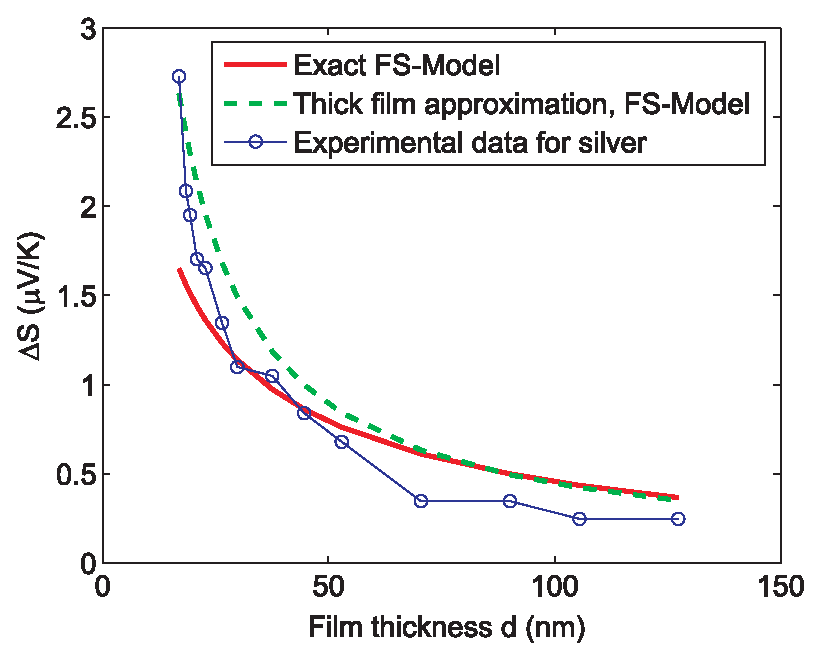
\includegraphics[width=.95\columnwidth,clip]{figures/SNMRn} } % Silver_NarasimhaMohanReddy
\caption{Difference of the Seebeck coefficient between the bulk material and a thin film with thickness $d$ for silver, $\lambda = 56\,  \mathrm{nm}$ \cite{hubin1974resistivity},  $p_s = 0.3$, $E_\mathrmm{F} = 5.5\, \mathrm{eV}$ \cite{ibach2003solid}, $T = 273\, \mathrm{K}$; other parameters and measurement data from \cite{rao1977size}.}
\label{fig:FigSilver}
\end{figure}

\begin{figure}[h]
\centerline{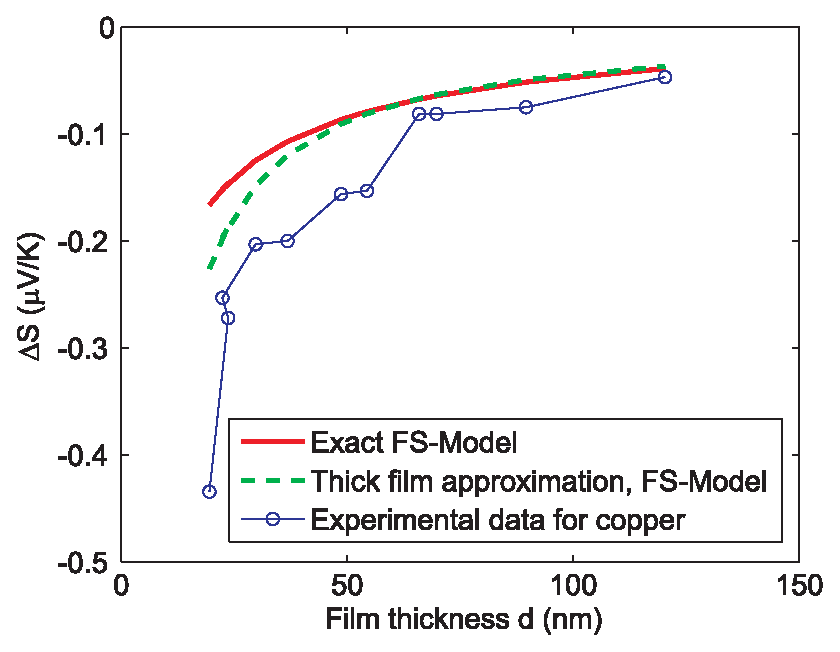
\includegraphics[width=.95\columnwidth,clip]{figures/CNMRn} } % Copper_NarasimhaMohanReddy
\caption{Difference of the Seebeck coefficient for copper, $\lambda = 41\, \mathrm{nm}$, $p_s = 0.3$, $E_\mathrmm{F} = 7.0\, \mathrm{eV}$ \cite{ibach2003solid}, $T = 273\, \mathrm{K}$; other parameters and measurement data from \cite{rao1976electrical}.}
\label{fig:FigCopper}
\end{figure}
%

However, the weak slope of the curve of the exact calculation
based on (\ref{Sf}) produces a large error for a thickness below the electron mean free path. This implies that the Fuchs-Sondheimer model is an inadequate description of the very thin film behaviour. It is surprising that the thick film approximation curve shows a better agreement than the exact curve since it is only valid for $k \gg1$. The opposite sign of $\Delta S$ for copper and silver is due to the different energy dependence of the electron mean free path.

It should be pointed out that the Fuchs-Sondheimer model only provides a good match with experiment for extremely rough surfaces ($p_s=0$ is a perfectly rough surface) according to \cite{sambles1983resistivity}. But a more critical problem is the availability of a complete set of measurement data including all transport parameters for different metals providing consistent results. In summary the presented data fits relatively well the measurements of Narasimha Rao, Mohan, and Reddy for a monocrystalline film with a rough surface. For very thin films, a more accurate model is needed that also takes quantum effects into account to describe the size effect more precisely.

In the case of wires an approximate formula for thick wires (width and height greater than the electron mean free path) of arbitrary cross-section was developed by Dingle \cite{dingle1950electrical} for the wire conductivity $\sigma_\mathrmm{w}$, given by
\begin{equation}
\sigma_\mathrmm{w} = \sigma_\mathrmm{0} \left[ 1 - \frac{3}{16}(1 - p_s) \frac{P}{S} \lambda(E) \right] \, .
\end{equation}
Here, $P$ is the perimeter and $S$ is the wire cross-section area. By inserting above formula for the wire conductivity into the general expression for the Seebeck coefficient $(-\pi^2 k_\mathrmm{B}^2 T /3e E_\mathrmm{F}) \left(  \partial\ln \sigma /\partial\ln E\right)
|_{E=E_{\mathrmm{F}}} \ $ and taking into account the energy dependence of the electron mean free path, we obtain 
\begin{equation} \label{S_wire}
S_\mathrmm{w} = -\frac{\pi^2 k_\mathrmm{B}^2 T}{3e E_\mathrmm{F}} \left( V_\mathrmm{g} + \alpha U_\mathrmm{g}  \right)
\end{equation}
with the geometry factor 
\begin{equation}
\alpha =  1 - \frac{\frac{3}{16} (1 - p_s) \frac{P}{S}}{\frac{1}{\lambda}  - \frac{3}{16} (1 - p_s) \frac{P}{S}}  \,  .
\end{equation}
As expected, (\ref{S_wire}) can be simplified to (\ref{k>>1}) for films with thicknesses $d\gg \lambda$. For single-metal NTCs with different wire cross sections, one has to subtract the Seebeck coefficients of the two single wires with different geometry factors $\alpha_\mathrm{1} \text{ and } \alpha_\mathrm{2} $, yielding
\begin{equation} \label{S_NTC}
S_\mathrm{NTC} = -\frac{\pi^2 k_\mathrmm{B}^2 T}{3e E_\mathrmm{F}} \left( \alpha_\mathrmm{1} - \alpha_\mathrmm{2}\right) U_\mathrmm{g} \, .
\end{equation} 
This formula is evaluated based on two available measurement results for Pd/Pd single-metal NTCs with a height of 45\,nm and widths of 80\,nm/470\,nm \cite{russer_nanostructured_2015} and 50\,nm/200\,nm (Section \ref{Measurements} of this paper), respectively. The measured Seebeck coefficients for these two NTCs are $S_\mathrm{NTC} = 1.11\,\mu$V/K \cite{russer_nanostructured_2015} and $0.86\,\mu$V/K, respectively.
\begin{figure}[h]
\centering
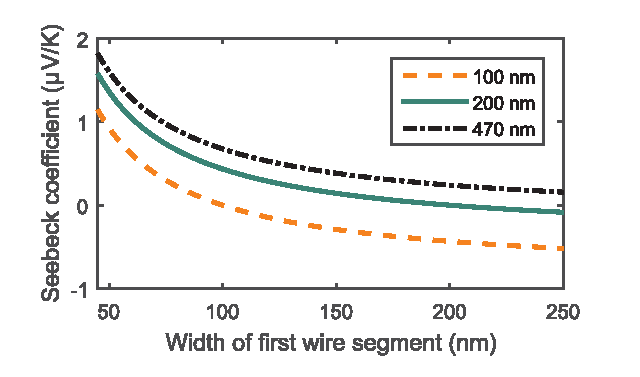
\includegraphics[width=1\columnwidth,clip]{figures/SMNTCSeebeckN.eps}
\caption{Calculated Seebeck coefficient of the single-metal NTC as a function of width of the first wire segment for various widths of the second wire segment. The height is 45\,nm, $U_\mathrmm{g}$ is set to 17.22.}
\label{fig:SMNTCSeebeck}
\end{figure}
In the following, we assume the parameter values $T = 300$ K, $E_\mathrmm{F} = 7.08$ eV \cite{mueller1970electronic}, $\lambda_F = 25.5$ nm, and $\mathrmm{p_s} = 0.6$. The material parameters $p_s$ and $\lambda$ are taken from \cite{shivaprasad1980electrical}, but vary with the production process conditions as discussed above. From (\ref{S_NTC}), we obtain $ U_\mathrmm{g} = 22.78$ and $11.66$ by using the data of the first and second thermocouple, respectively. This uncertainty in the exact value of $U_\mathrmm{g}$ may again be partially due to the production process conditions, as also discussed above in the context of Table \ref{tab:UgVgValues}. In addition, substrate effects and the fact that the wire segments are connected at a 90$^{\circ}$ angle at the hot junction, as discussed in Section \ref{Fabrication}, affect the measurement results, but are not explicitly considered in the theoretical model. Thus, fitting (\ref{S_NTC}) to the measurement results yields an effective value for $U_\mathrmm{g}$, which also accounts for these effects. Figure \ref{fig:SMNTCSeebeck} shows the geometry dependence of the Seebeck coefficient, where we here take the averaged value $ U_\mathrmm{g} = 17.22$.

From Figs. \ref{fig:FigSilver}, \ref{fig:FigCopper},  and \ref{fig:SMNTCSeebeck} it can be concluded that the efficiency of the NTC is maximized when a thin segment, with a thickness on the order of the electron mean free path, is connected to bulk material or to dimensions which are much greater than the electron mean free path. A large geometrical difference of the two segments leads to a large relative Seebeck coefficient and thus, according to (\ref{SVoltage}), to a higher Seebeck voltage. Quantum size effects beyond the electron mean free path length could improve the Seebeck coefficient even more and should be further investigated. 
%
%
%-----------------------------------------------------------------------------------------------------------------------------------------------------------------------
%
\section{Fabrication of the Antenna-Coupled \\ Single-Metal Nanothermocouple}\label{Fabrication}
%
%-----------------------------------------------------------------------------------------------------------------------------------------------------------------------
%
Now we present the fabrication method of single-metal ACNTCs using the same metal, both for the antenna and the NTC. Figure~\ref{fig1}a shows that the hot junction of the NTC is located at the center of the antenna, where the radiation-induced antenna current is at maximum and hence the heating is largest. The hot junction of the NTC is formed from a junction of a narrow and wide wire segments from the same metal. The single-metal NTC operation is based on the structure size dependence of the absolute Seebeck coefficient in nanowires~\cite{szakmany_single-metal_2014}. When the mean free path of electrons are comparable to the physical dimensions of a conductor, the absolute Seebeck coefficient is decreased from its bulk value due to the increased electron scattering. We exploit this property for single-metal NTCs by constructing them from the same metal nanowires, but with two different cross sections. As a result, the relative Seebeck coefficient between the two wire segments is non zero, because the reduction of the absolute Seebeck coefficient is more pronounced in the narrow wire segment.

%
\begin{figure}[h]
\centerline{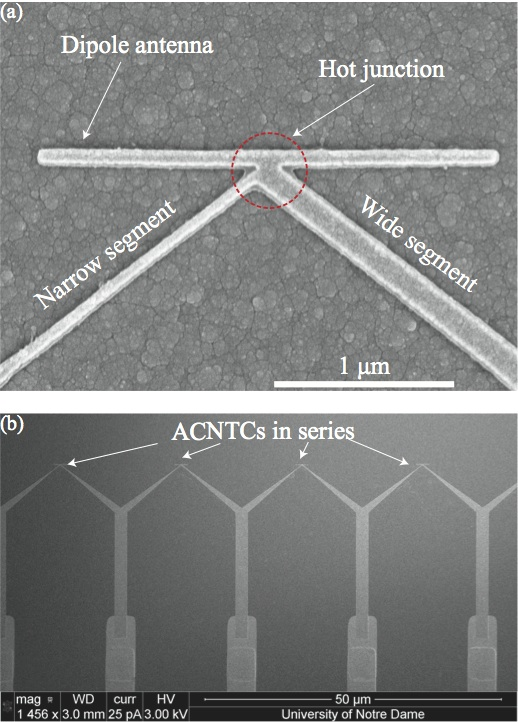
\includegraphics[width=0.95\columnwidth,clip]{figures/Fig3new}}
\caption{Scanning electron micrograph of (a) an ACTC and (b) a thermopile constructed from several ACTCs connected in series.}
\label{fig1}
\end{figure}
%

Similar to our previous work~\cite{szakmany_single-metal_2014, szakmany_antenna_2013, szakmany_nanowire_2013}, the antenna-coupled single-metal nanothermocouples were patterned by electron beam lithography, and metalized by 45-nm-thick electron beam evaporated Pd. The 50 nm and 200 nm wide wire segments are joined at 90 deg at one end, and connected to the bonding pads at their other ends as shown in Fig.~\ref{fig1}.
The dipole antenna, which is 2.4~$\mu$m long, is connected to the NTC at its center. The measured electrical resistance of these devices is 2.1 k$\Omega$. Fabrication complexity of such devices is greatly reduced compared to bi-metallic ACNTCs~\cite{szakmany_antenna_2013}, since only one lithography and one deposition step is required.

We constructed antenna-coupled thermopiles by connecting several ACNTCs in series to increase the output voltage of the detector. Figure~\ref{fig1}b shows such a linear thermopile array, where each individual ACNTC possesses its own read-out circuit, allowing thermopile-length-dependent measurements. 
%-----------------------------------------------------------------------------------------------------------------------------------------------------------------------
%
\section{Thermal Conduction}\label{ThermalConduction}
%
%-----------------------------------------------------------------------------------------------------------------------------------------------------------------------
%
%
For the purpose of investigating the thermal heat conduction, we approximate the TC structure by  a circular thermocouple patch. This patch models the hot junction of the ACTC. The patch is sitting on a substrate, its diameter is 2$r_0$, and its thickness is $d_0$ as shown in Fig.~\ref{fig.disk}.
%
\begin{figure}[h]
\centerline{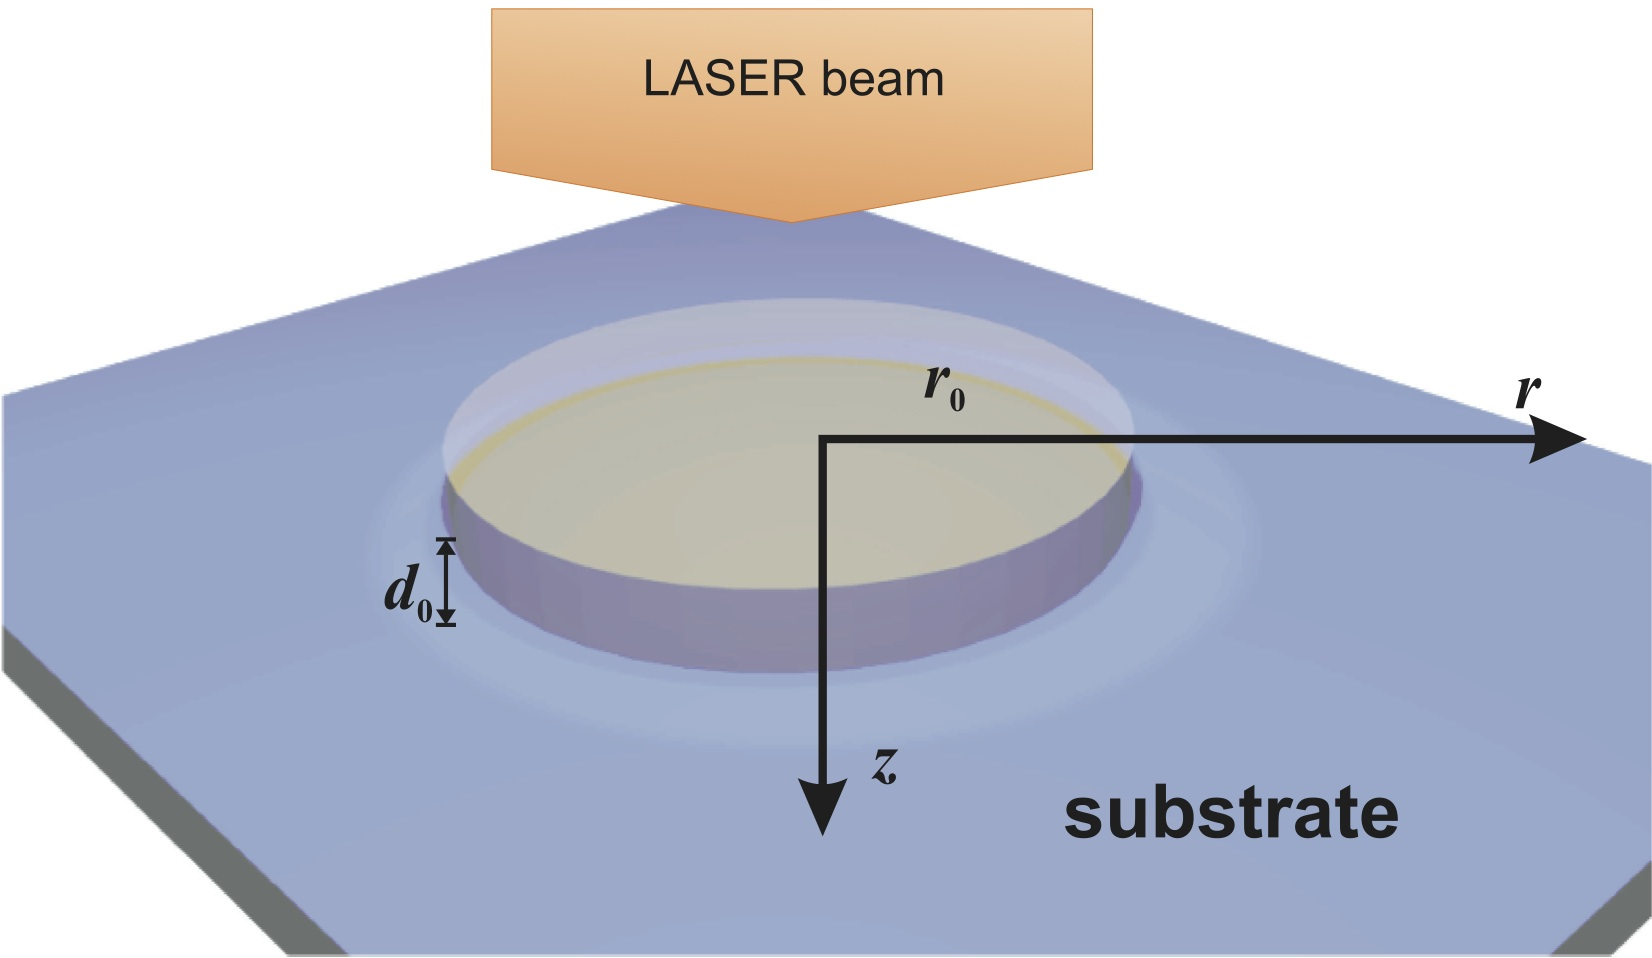
\includegraphics[width=0.85\columnwidth,clip]{figures/TC_fig2}}
\caption{Perspective view on the disk with heated patch.}
\label{fig.disk}
\end{figure}
%
Excited by an impulsive heating by the patch at time $t=0$, the temperature time dependence at $r=z=0$ is obtained for this structure by solving the diffusion equation~\cite{russer_nanostructured_2015} as
%
\begin{align} 
	T(0,0,t)  & =  \frac{2r_0}{\pi}T_0 \! \int_{0}^\infty  \!  \frac{d_0}{1+(\eta d_0)^2} \, e^{-\alpha \eta^2  t}  d \eta  \; \times \nonumber \\
	 &  \int_{0}^\infty  \!  J_1(\beta r_0)\, e^{-\alpha \beta^2  t}  d \beta  \, .
	\label{heat015}
\end{align}
%
The thermal diffusivity obtained for silicon as substrate material is $\alpha=9.078\times10^{-5}$m$^2$s$^{-1}$, considering a thermal conductivity $k=148$~Wm$^{-1}$K$^{-1}$, density $\rho=2329$ kg m$^{-3}$, and specific heat $c_p=700$ J~kg$^{-1}$K$^{-1}$. We have varied the circular patch radii $r_0$ and have assumed an initial penetration depth $d_0=10$~nm at $r=0$~nm, $z=0$~nm. The time dependence of $\Delta T$ obtained is plotted in Fig.~\ref{product02c1} and shows that $\Delta T$ is independent of $r_0$ for small times below 1~ps. In this case, the time evolution is predominantly determined by diffusion in $z$-direction. As time advances, and spatial extension of the diffusion spread of $\Delta T$ gets on the order of $r_0$, we find a strong dependence of the time evolution of $\Delta T$ on the junction radius $r_0$.

%
\begin{figure}[h]
\centering
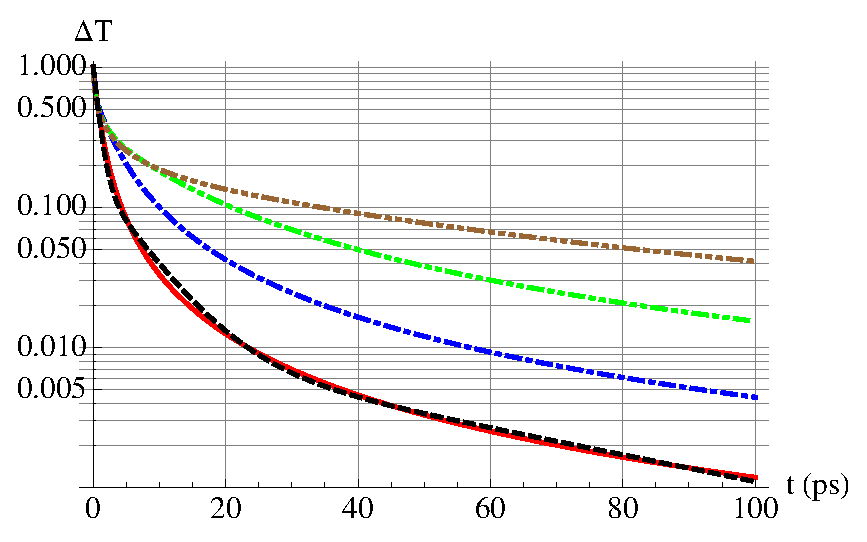
\includegraphics[width=1\columnwidth,clip]{figures/product02c1newn2.eps} \\
\caption{Time dependence of $\Delta T$ (normalized) for variable  circular patch radius $r_0 $, %\newline  
for an initial penetration depth $d_0=10$~nm at $z=0$~nm for $r_0=25$~nm
\textcolor{red}{\bf --------}, $r_0=50$~nm \textcolor{blue}{\bf --~-~--~-}, $r_0=100$~nm \textcolor{green}{\bf --~-~-~--~-~-},   $r_0=200$~nm \textcolor{brown}{\bf --~-~-~-~--} computed from (\ref{heat015})  and from the Foster topology equivalent circuit (Fig.~\ref{fig.RCcircuit}b) for $r_0=25$~nm \textcolor{black}{\bf ~--~--~--}.} 
\label{product02c1}
\end{figure}
%
In order to model the dynamics of the TC we have implemented in a previous work~\cite{szakmany_nano-antenna_2014} an equivalent circuit which accounted, using a single $RC$ element, for the temperature decay with a single time constant. A single time constant, however, is not sufficient for modeling the thermal subsystem accurately, since there are several regions with variable heat capacity and variable heat conductivity which govern the process. Hence, introducing several time constants will improve accuracy~\cite{szekely_evaluation_1997}. Using Foster or Cauer equivalent circuit topologies, we can synthesize lumped element equivalent circuit models with the desired accuracy~\cite{szekely_fine_1988, gerstenmaier_combination_2007}.


%
\begin{figure}[h]
\centerline{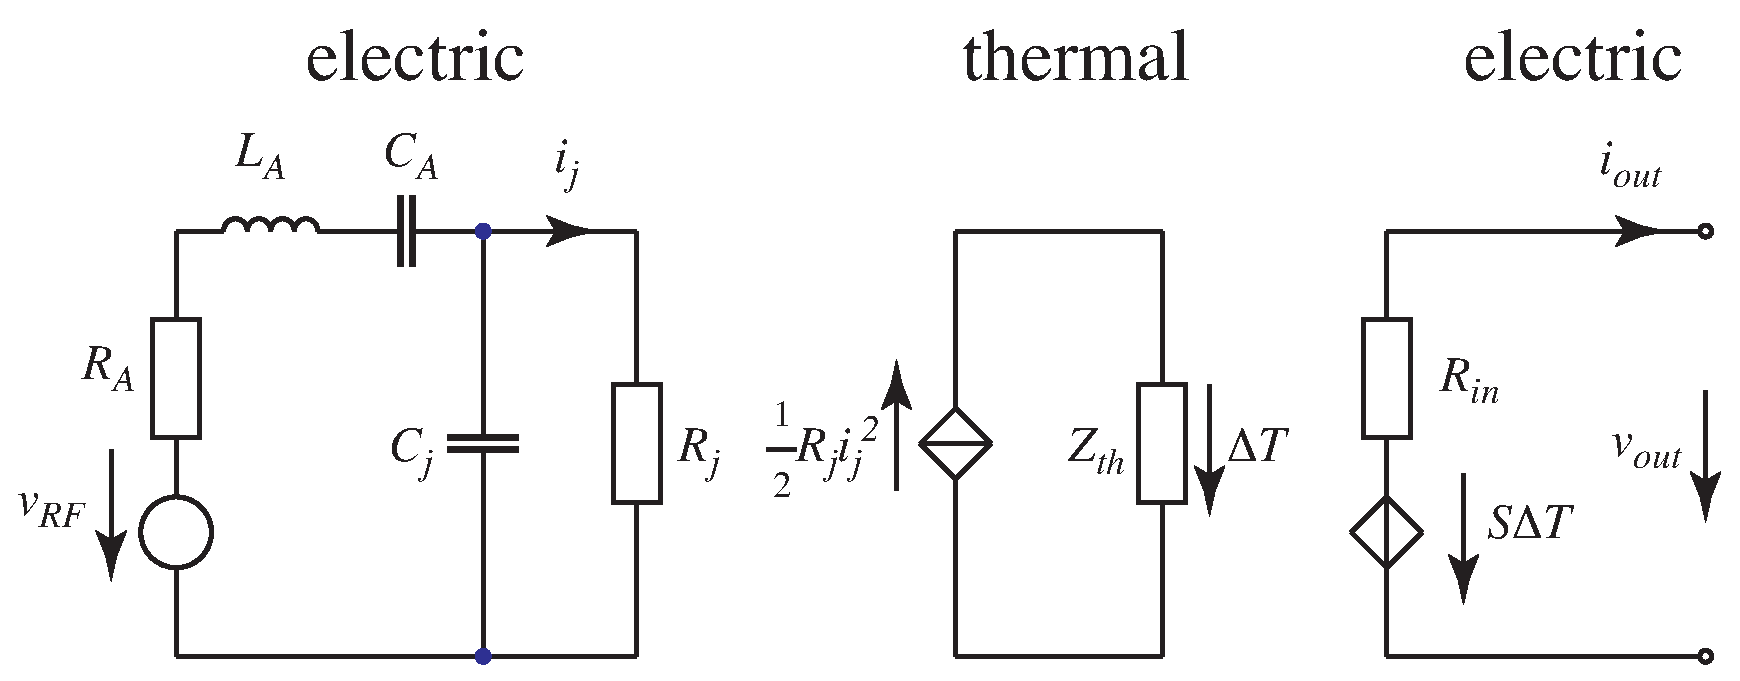
\includegraphics[width=0.95\columnwidth,clip]{figures/thermocouple_circuit03a.eps}}
\caption{Equivalent circuit of the thermocouple.}
\label{fig.circuit}
\end{figure}
%
The TC is model by an equivalent circuit consisting of three parts, as shown in Fig.~\ref{fig.circuit}: the left-hand side models the electric $RF$ (radio frequency) part, the center part represents the thermal equivalent circuit, and on the right-hand side, the equivalent circuit for the electric $LF$ (low frequency) part is given. The antenna's open-circuit voltage, caused by the incident $RF$ electrical field, is denoted as $v_{RF}$, and its radiation resistance, its inductance, and capacitance are denoted as $R_A$, $L_A$, and $C_A$, respectively. Joule heating occurs in the TC junction due to the dissipation of the $RF$ power $\frac{1}{2} I_j^2 R_j$, where $R_j$ is the junction resistance and $i_j$ is the $RF$ current in the junction resistance. The junction capacitance is denoted as $C_j$. The dissipated power controls the current in the thermal equivalent circuit which governs together with the thermal impedance $Z_{th}$ the temperature enhancement $\Delta T$. This temperature enhancement induces a Seebeck voltage $S \Delta T$ in the circuit modeling the electric low-frequency part. The inner resistance for the LF circuit model is $R_{in}$.
%
\begin{figure}[h]
\centerline{\includegraphics[width=0.95\columnwidth,clip]{figures/equivalent_circuit01.pdf}}
\caption{Circuit modeling the thermal transfer function of the thermocouple: {a) Cauer type RC equivalent circuit, b) Foster type RC equivalent circuit.}}
\label{fig.RCcircuit}
\end{figure}
%
Having obtained the solution of the diffusion equation, $RC$ equivalent circuits can be used to model the thermal impedance $Z_{th}$. For this purpose we have to consider the frequency poles of this solution.  In the complex frequency plane, the poles are located on the negative real axis. 

Two topologies for lumped element equivalent circuits are depicted in Fig:~\ref{fig.RCcircuit}: The Cauer type topology (a) yields a ladder network with capacitors and resistors as the parallel and the series elements, respectively. The Foster type topology (b) yields parallel $RC$-circuits connected in series.

For the Cauer topology equivalent circuit, given in Fig.~\ref{fig.RCcircuit}a, the thermal impedance $Z_{th}$ is of the form
%
\begin{equation} \label{thermalimpedance01}
	Z_{th}(p) = \frac{1}{p C_{th1}+\frac{1}{{R_{th1}+\frac{1}{p C_{th2}+\frac{1}{R_{th2}+\frac{1}{p C_{th3}+\frac{1}{{R_{th3}+ \cdots}}}}}}}} \, ,
\end{equation}
%
where $p$ is the complex frequency. 


%
The impedance $Z_{th}$ of the Foster topology equivalent circuit (Fig.~\ref{fig.RCcircuit}b) is given by
%
\begin{equation} \label{thermalimpedance02}
	Z_{th}(p) = \sum_{i=1}^n\frac{R_{thi}}{1+ p \tau_i }
\end{equation}
%
with the time constant $\tau_i = R_{thi}C_{thi}$. The pulse response  is the inverse Fourier transform of $Z_{th}(p)$, given  by
%
\begin{equation}
	z_{th}(t) = \sum_{i=1}^n  R_{thi}e^{-\frac{t}{ \tau_i }} \, .
\end{equation}
%

We used the analytic solution (\ref{heat015}) to obtain the thermal time response of the TC with parameters stated above, and we compared these results to the matched equivalent Foster topology model. The equivalent circuit model exhibits three $RC$ elements with $R_1=0.85 R_0$, $\tau_1 = 0.87$~ps, $R_2=0.14 R_0$, $\tau_2 = 6.33$~ps, $R_3=0.01 R_0$, $\tau_3 = 45.5$~ps. This comparison is given in Figure~\ref{product02c1}.

%
%-----------------------------------------------------------------------------------------------------------------------------------------------------------------------
%
\section{THz Detectors and Mixers}\label{Detector}
%
%-----------------------------------------------------------------------------------------------------------------------------------------------------------------------
%
Consider the equivalent circuit of the thermocouple depicted in Fig.~\ref{fig.circuit}. This circuit represents a quadratic detector. The right-hand and left-hand electric equivalent circuits are linear, whereas the thermal circuit in the center exhibits quadratic transfer characteristics. The left-hand electric equivalent circuit can be described in frequency domain by
%
\begin{equation}	\label{eqdet010}
	\left[\begin{array}{c}V_{rf} \\0\end{array}\right] = \Mbf{Z}_{rf} \left[\begin{array}{c}I_{rf} \\ - I_j\end{array}\right]
\end{equation}
%
\begin{equation}	\label{eqdet020}
	\Mbf{Z}_{rf} = \left[\begin{array}{cc}R_A+pL_A+ \frac{1}{pC_A}+ \frac{1}{pC_j} & \frac{1}{pC_j} \\
	                                                        \frac{1}{pC_j} & R_j + \frac{1}{pC_j}
	                       \end{array}\right] \, .
\end{equation}
%
This yields
%
\begin{equation}	\label{eqdet030}
  I_j = \frac{pC_j}{\left(1+\frac{C_j}{C_A} + p R_A C_j + p^2 L_A C_j\right)\left(1+ pR_jC_j\right) - 1} V_{rf} \, .
\end{equation}
%
For the case of negligible junction capacitance $C_j \rightarrow 0$ we obtain
%
%
\begin{equation}	\label{eqdet040}
  I_j = \frac{1}{R_A+R_j + pL_A + 1/pC_A} V_{rf} \, .
\end{equation}
%
In the tuned case $\omega L_A = 1/ \omega C_A$ with harmonic excitation $p = \jmath \omega$ we obtain
%
\begin{equation}	\label{eqdet050}
  I_j(p) = \frac{1}{R_A+R_j } V_{rf}(p) \, .
\end{equation}
%


The square-law rectification is accomplished in the thermal part of the equivalent circuit. The heat $q$ generated in the thermocouple junction with the electric resistance $R_j$ is related to the flowing electric current via
%
\begin{equation}	\label{eqdet060}
	\frac{dq(t)}{dt} = \frac{1}{2} R_j i_j^2(t)\, .
\end{equation}
%
In the complex frequency domain this equation becomes
%
\begin{equation}	\label{eqdet070}
	\jmath \omega Q (\omega) = \frac{1}{2} R_j \left(I_j(\omega) \ast I_j(\omega) \right) \, ,
\end{equation}
%
where $I_j(\omega)$ and $Q(\omega)$ are the electric junction current and the heat, respectively in the frequency domain and the operator $\ast$ denotes the convolution operation.
The time derivation is considered as a thermal current and the temperature increase $\Delta T(t)$ as a thermal voltage. Its Fourier transform we denote with $\Delta \tilde{T}(\omega)$. The temperature increase due to the heat $Q (\omega)$ is given by
%
\begin{equation}	\label{eqdet080}
	\Delta \tilde{T}(\omega) = \jmath \omega Q (\omega) Z_{th}(\omega) \, ,
\end{equation}
%
where the thermal impedance  $Z_{th}(\omega)$ is given by (\ref{thermalimpedance01}) or  (\ref{thermalimpedance02}), respectively.

The right-hand electric equivalent circuit in Fig.~\ref{fig.circuit} is the linear circuit describing the intermediate frequency or low-frequency output. The controlled voltage source $S \Delta T$ accounts for the thermal voltage excited via the Seebeck effect. The output voltage $V_{out}(\omega)$ is given by
%
\begin{equation}	\label{eqdet090}
	V_{out}(\omega) = S \Delta \tilde{T}(\omega) - R_{in} I_{out} (\omega)\, .
\end{equation}
%
Inserting (\ref{eqdet080}),  (\ref{eqdet070}), and (\ref{eqdet050}) yields
%
\begin{equation}	\label{eqdet100}
	V_{out}(\omega) =  \frac{S  Z_{th}(\omega) R_j}{2(R_A+R_j )^2} \left(V_{rf}(\omega)  \ast V_{rf}(\omega)  \right)  - R_{in} I_{out} (\omega)\, .
\end{equation}
%
The open-circuit output voltage $V_{out,0}(\omega)$ for $I_{out} (\omega)=0$ is given by
%
\begin{equation}	\label{eqdet110}
	V_{out,0}(\omega) =  \frac{S  Z_{th}(\omega) R_j}{2(R_A+R_j )^2} \left(V_{rf}(\omega) \ast V_{rf}(\omega)  \right) \, .
\end{equation}
%
Figure~\ref{fresponsec01} shows 
%
\begin{figure}[h]
\centering
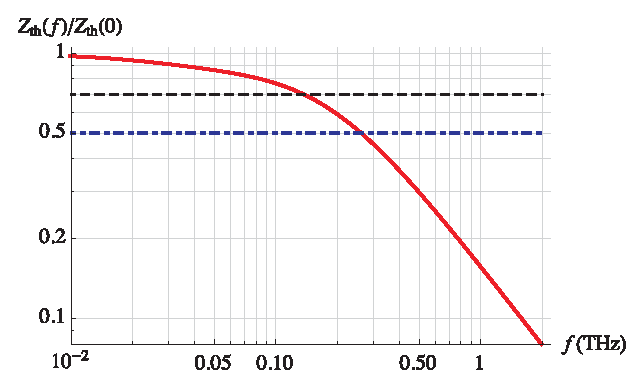
\includegraphics[width=1.0\columnwidth,clip]{figures/fresponsec01n.eps} \\
\caption{Frequency response $Z_{th}(f)/Z_{th}(0)$ for a circular patch radius $r_0 =25$~nm computed from the Foster topology equivalent circuit (Fig.~\ref{fig.RCcircuit}b) using (\ref{thermalimpedance02}); 3 dB cutoff frequency marker for mixer \textcolor{black}{\bf --~--~--} and detector \textcolor{blue}{\bf --~-~--~-} mode.} 
\label{fresponsec01}
\end{figure}
%
the frequency response $Z_{th}(f)/Z_{th}(0)$ for a circular patch radius $r_0 =25$~nm computed from the Foster topology equivalent circuit (Fig.~\ref{fig.RCcircuit}b) using (\ref{thermalimpedance02}). 
The equivalent circuit model exhibits three $RC$ elements with $R_1=0.85 R_0$, $\tau_1 = 0.87$~ps,  $R_2=0.14 R_0$, $\tau_2 = 6.33$~ps, $R_3=0.01 R_0$, $\tau_3 = 45.5$~ps. For the chosen parameters the computed 3~dB cutoff frequency is 136.6~GHz in the mixer mode and 206.8~GHz in the detector mode.
%

Due to the broad-band characteristics at the \emph{rf} the thermocouple is perfectly suited for mixer applications for frequencies up to 30~THz. Consider an  \emph{rf} input signal voltage $v_1(t)$ with the carrier frequency $\omega_1$ amplitude modulated with the signal  $a_1(t)$,
%
\begin{equation}	\label{eqmix010}
	v_1(t) =  a_1(t)\cos(\omega_1 t +\varphi_1) \, .
\end{equation}
%
The Fourier transform of $v_1(t)$ is symbolically denoted by
%
\begin{equation}	\label{eqmix012}
	v_1(t) \TDFD V_1(\omega) \, 
\end{equation}
%
and defined via
%
\begin{equation}	\label{eqmix014}
	V_1(\omega) = \int_{-\infty}^\infty v_1(t) e^{-\jmath \omega t} dt \, .
\end{equation}
%
From (\ref{eqmix010}), (\ref{eqmix012}), and (\ref{eqmix014}) we obtain
%
\begin{equation}	\label{eqmix016}
	V_1(\omega) = \frac{1}{2} A_1(\omega+ \omega_1) e^{\jmath \varphi_1} +\frac{1}{2} A_1(\omega- \omega_1)e^{-\jmath \varphi_1}\, .
\end{equation}
%
We superimpose a harmonic local oscillator signal
%
%\begin{equation}	\label{eqmix020}
	$v_0(t) =  b_0 \cos(\omega_0 t +\varphi_0) \, .$
%\end{equation}
%
Its Fourier transform is
%
\begin{equation}	\label{eqmix020}
	V_0(\omega) = \frac{b_0}{2}   \left[\delta(\omega - \omega_0) e^{-\jmath \varphi_0} + \delta(\omega + \omega_0) e^{\jmath \varphi_0}\right]\, .
\end{equation}
%
The total input signal of the thermocouple is
%
\begin{align}	\label{eqmix030}
	v_{rf}(t)  & = v_0(t) + v_1(t) \\
	              & = a_1(t)\cos(\omega_1 t +\varphi_1) +  b_0 \cos(\omega_0 t +\varphi_0) \, . \nonumber
\end{align}
%
This yields in the frequency domain
%
\begin{align}	\nonumber
	V_{rf}(\omega) & =  \frac{1}{2} A_1(\omega+ \omega_1) e^{\jmath \varphi_1} +\frac{1}{2} A_1(\omega- \omega_1)e^{-\jmath \varphi_1} \\  
	              &                                       +  \frac{b_0}{2}   \left[\delta(\omega - \omega_0) e^{-\jmath \varphi_0}) + \delta(\omega + \omega_0) e^{\jmath \varphi_0})\right] \, . \label{eqmix040} 
\end{align}
%
The Fourier transform of the product of two signals $s_a(t)$ and $s_b(t)$ is given by the convolution of the respective spectra, i.e.,
%
\begin{equation}	\label{eqmix032}
	s_a(t) s_b(t) \FDTD S_A(\omega) \ast S_B(\omega)\, ,
\end{equation}
%
where the convolution $S_A(\omega) \ast S_B(\omega)$ is defined by
%
\begin{equation}	\label{eqmix034}
%\left[ S_A(\omega) \ast S_B(\omega) \right] (\omega)  
S_A(\omega) \ast S_B(\omega)  = \left[ S_A \ast S_B \right] (\omega)
	 = \Int S_A(\omega') S_B(\omega-\omega') d \omega' \, . 
\end{equation}
%
We note 
%
\begin{align}	\label{eqmix036}
S_A(\omega-\omega_1) &  \ast S_B(\omega-\omega_2)  = \\
= & \Int  S_A(\omega' -\omega_1) S_B(\omega-\omega' -\omega_2) d \omega' \nonumber \\
= & \left[ S_A \ast S_B \right] (\omega-\omega_1-\omega_2) \, . \nonumber
\end{align}
The autoconvolution of $V_{rf}(\omega)$ is given by
%
\begin{align}	\label{eqmix040}  
	& V_{rf}(\omega) \ast V_{rf}(\omega) =  \frac{1}{2} \left[A_1\ast A_1\right](\omega) +\frac{b_0^2}{2} \delta(\omega) \\
			%&+ \left[A_1\ast A_1\right](\omega-\omega_1+\omega_0) +\frac{b_0^2}{2} \delta(\omega) \nonumber \\
	                &      +  \frac{b_0}{4}\left[ A_1(\omega + \omega_1 -\omega_0 )e^{\jmath (\varphi_1-\varphi_0)} \right. \nonumber \\
	                &\left.+ A_1(\omega - \omega_1 +\omega_0 )e^{-\jmath (\varphi_1-\varphi_0)} \right]  \nonumber \\
	                &      +  \frac{b_0}{4}\left[ A_1(\omega + \omega_1 +\omega_0 )e^{\jmath (\varphi_1+\varphi_0)} \right. \nonumber \\
	                &\left.+ A_1(\omega - \omega_1 -\omega_0 )e^{-\jmath (\varphi_1+\varphi_0)} \right]  \nonumber \\	                
	                 &+   \frac1{4} \big( \hspace{-0.8mm}\left[A_1\ast A_1\right](\omega+2\omega_1) e^{\jmath 2\varphi_1} %\nonumber \\ 
	                % &      
	                %+ \frac1{4} 
	                \hspace{-0.8mm}+\left[A_1\ast A_1\right](\omega-2\omega_1) e^{-\jmath 2\varphi_1} \big)\nonumber \\  
	                &      +  \frac{b_0^2}{4}\left[ \delta(\omega -2\omega_0) e^{-\jmath 2\varphi_0} + \delta(\omega +2\omega_0)e^{-\jmath 2\varphi_0}\right] \nonumber 
	                \, . 
\end{align}
%
Assuming the magnitude of the frequency difference $|\omega_1- \omega_0|$ to be small compared to the frequencies $\omega_1$ and $\omega_0$ we have in the first line of (\ref{eqmix040}) the low-frequency and dc components of the direct rectification of the signal $V_1$ and the local oscillator signal $V_0$. The second and third lines exhibit the intermediate frequency part with frequencies around $|\omega_1- \omega_0|$ and the lines 4 to 7 contain spectral parts around twice the local oscillator frequency, i.e., around $2\omega_0$. These frequencies around $2\omega_0$ are filtered out by $Z_{th}(\omega)$. We need only to consider the low-frequency part playing a role in direct detector applications
%
\begin{align}	\label{eqmix050}  
	\left. V_{rf}(\omega) \ast V_{rf}(\omega) \right|_{lf} & =  \frac{1}{2} \left[A_1\ast A_1\right](\omega)  +\frac{b_0^2}{2} \delta(\omega) 	                \,  
\end{align}
%
and the intermediate frequency part playing a role in mixer applications
%
\begin{align}	\label{eqmix060}
	\left. V_{rf}(\omega) \ast V_{rf}(\omega) \right|_{if}& = \frac{b_0}{4}\left[ A_1(\omega + \omega_1 -\omega_0 )e^{\jmath (\varphi_1-\varphi_0)} \right. \\
	& +  \left. A_1(\omega - \omega_1 +\omega_0 )e^{-\jmath (\varphi_1-\varphi_0)} \right] 
	\, . \nonumber
\end{align}
%
Inserting (\ref{eqmix050}) into (\ref{eqdet110}) yields the open-circuit output voltage $V_{out,lf,0}(\omega)$ for $I_{out} (\omega)=0$
%
\begin{equation}	\label{eqmix070}
	V_{out,lf,0}(\omega) =  \frac{S  Z_{th}(\omega) R_j}{2(R_A+R_j )^2} 
	 \left[ \frac{1}{2} \left[A_1\ast A_1\right](\omega)  +\frac{b_0^2}{2} \delta(\omega) \right]	 \, .
\end{equation}
%
The $lf$ output frequency characteristics of the detector is determined by $Z_{th}(\omega)$ and represented in Fig.~\ref{fresponsec01} for a NTC diameter of 25~nm, showing a detector $lf$ cutoff frequency equal to the thermal cutoff frequency  of 260.8 GHz. In general the expression $\left[A_1\ast A_1\right](\omega)$ denotes the spectrum of the square-law rectified AM signal envelope.

For the case of mixer operation we insert (\ref{eqmix060}) into (\ref{eqdet110}) and obtain the open-circuit output voltage $V_{out,if,}(\omega)$ 
%
\begin{align}	\label{eqmix080}
	V_{out,if,0}(\omega) &=  \frac{S  Z_{th}(\omega) R_j}{2(R_A+R_j )^2} 
	 \frac{b_0}{4}\left[ A_1(\omega + \omega_1 -\omega_0 )e^{\jmath (\varphi_1-\varphi_0)} \right. \\
	& +  \left. A_1(\omega - \omega_1 +\omega_0 )e^{-\jmath (\varphi_1-\varphi_0)} \right] 
	\, . \nonumber
\end{align}
%
The $rf$ signal with the frequency $\omega$ is shifted by the local oscillator frequency $\omega_0$ to the intermediate frequency $|\omega-\omega_0|$. The intermediate frequency band again is limited by the thermal cutoff frequency of 136.6 GHz. In the mixer case, the envelope spectrum $A_1(\omega)$ is frequency shifted but exhibits no nonlinear distortion.
%
%
%-----------------------------------------------------------------------------------------------------------------------------------------------------------------------
%
\section{Measurements}\label{Measurements}
%
%-----------------------------------------------------------------------------------------------------------------------------------------------------------------------
%
Infrared measurements of the devices were performed by a linearly polarized CO$_2$ laser operating at 28.3 THz. The laser beam was square wave modulated by a mechanical chopper at 1 kHz. In order to maximize the device response, the polarization angle of the laser beam was set parallel to the antenna axis by a half-wave plate. The open-circuit voltage response was measured by a custom made pre-amplifier and with standard lock-in techniques. The measurement set-up is shown in Fig.~\ref{figsetup}.

%
\begin{figure}[h]
\centerline{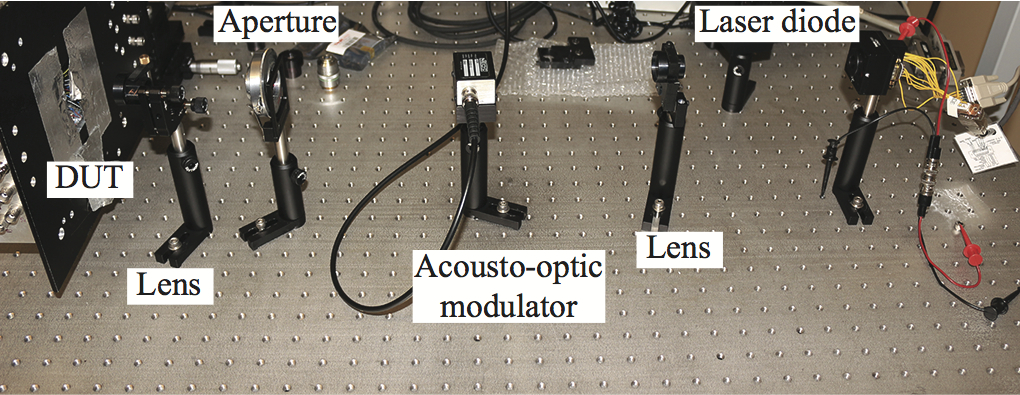
\includegraphics[width=1.0\columnwidth,clip]{figures/setup.jpg}}
\caption{Measurement set-up.}
\label{figsetup}
\end{figure}
%

We measured the open-circuit voltage response of the thermopile with various length, as shown in Fig.~\ref{fig2}. The response ($V_{th}$) followed the thermopile addition rule, i.e., $V_{th}$ is a linear function of the number of ACNTCs in the thermopile. This confirms our assumption that the radiation-induced antenna currents heat the hot junction of the NTC, and shows that antenna-coupled single-metal thermocouples and thermopiles function as IR detectors. The relative Seebeck coefficient is 0.86~$\mu$V/K, measured by the characterization platform introduced in~\cite{szakmany_nanowire_2013}, for a single-metal NTC constructed from 50 and 200 nm wide Pd wire segments.
%
\begin{figure}[h]
\centerline{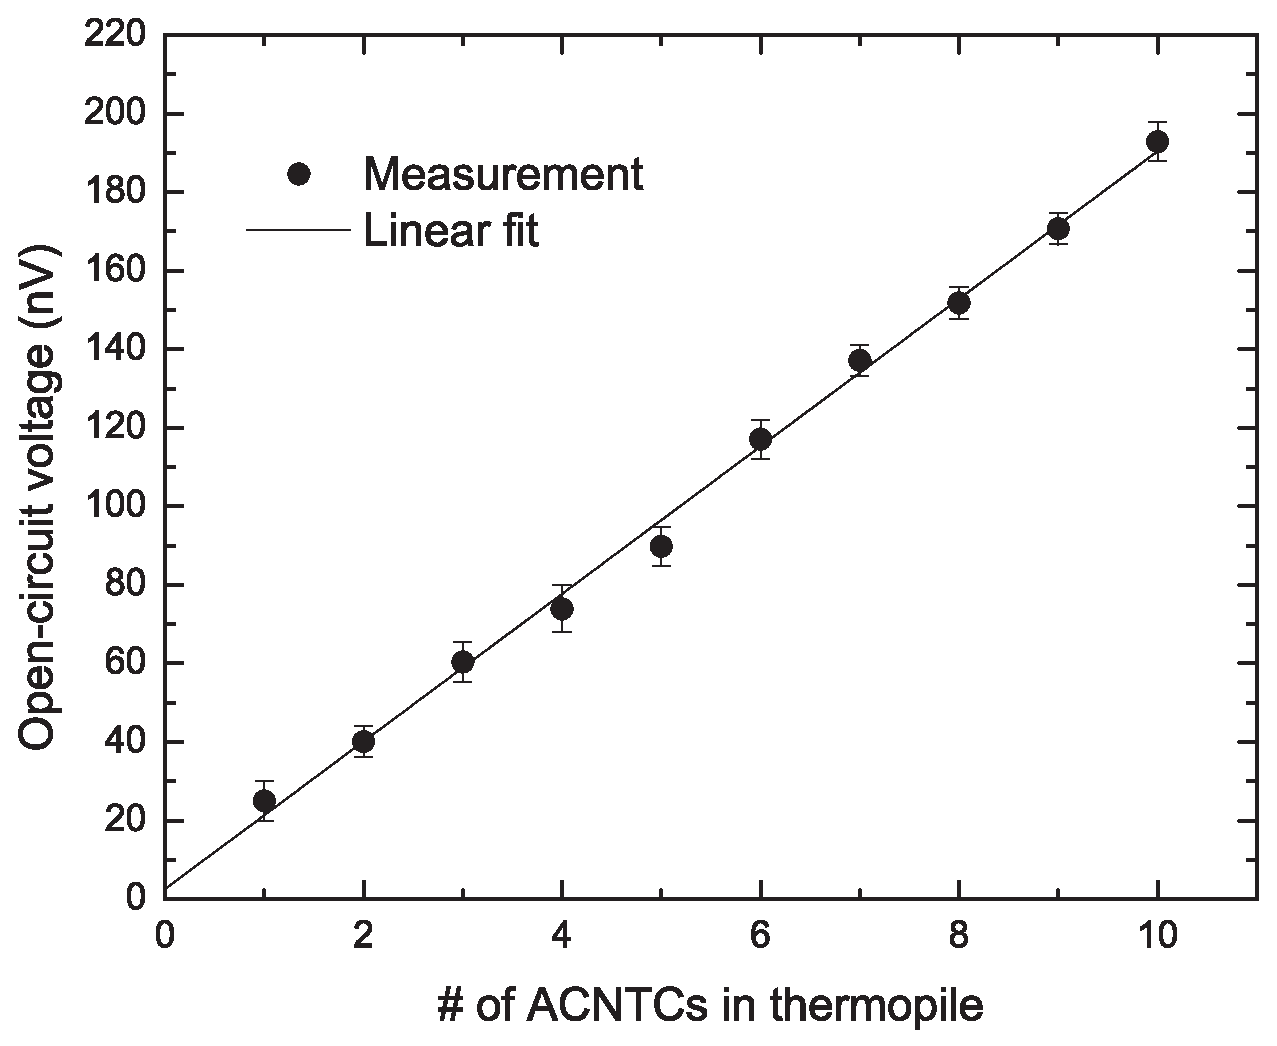
\includegraphics[width=0.95\columnwidth,clip]{figures/Fig10new}}
\caption{Open-circuit voltage as a function of thermopile length.}
\label{fig2}
\end{figure}
%

Our IR experimental setup does not allow direct measurement of the frequency-dependent response of ACNTCs. Therefore, the frequency-dependent response of the NTCs was determined by pulse heating of the hot junctions using an acousto-optic modulator and a laser diode. 

To characterize the frequency-dependent response of NTCs to pulsed heating, we built the structure shown in Fig.~\ref{fig3}. 
%
\begin{figure}[h]
\centerline{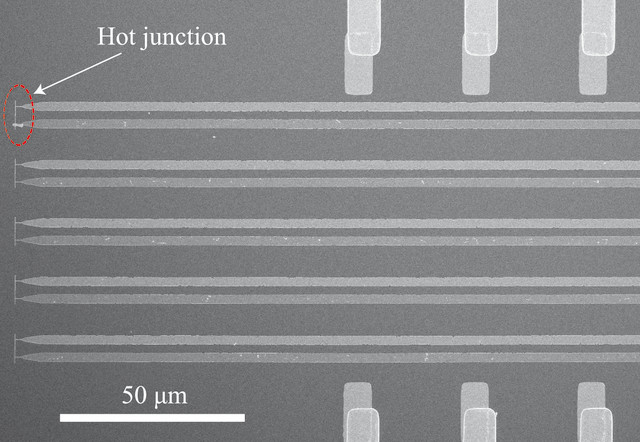
\includegraphics[width=1.0\columnwidth,clip]{figures/Fig3}}
\caption{Scanning electron micrograph of the NTCs for frequency-dependent measurements. The hot and cold (not shown) junctions are separated by 400~$\mu$m. A thermopile was constructed from the NTCs by connecting them in series at their terminals.}
\label{fig3}
\end{figure}
%
The geometry of the hot junctions is nominally identical in both structures (ACNTC and NTC), to avoid the impact of the thermal conductivity and geometry of the antenna on the response time of the NTC. The cold junctions for the frequency-dependent measurements are located 400~$\mu$m away from the hot junctions to ensure that the laser beam does not illuminate the cold junctions and so they remain at ambient temperature.
We also constructed a thermopile by connecting four NTCs in series at their terminals.

Now we discuss the various components of our experimental setup. Our heat source is an AlGalnP laser diode (HL6545MG), operating at 660~nm in a constant emission mode. The laser beam is collimated and focused to form a
200-$\mu$m-diameter spot at the devices, which was determined
by the widely-used knife edge measurement technique. 

In order to perform frequency-dependent measurement, the beam is square-wave modulated with an acousto-optic modulator (AOM) between 30 kHz and 6.5 MHz. The signal generated by the NTCs in response to the laser induced temperature oscillations, is detected by an SR844 high frequency lock-in amplifier, which was synchronized to the AOM driver. In order to avoid the intrinsic bandwidth limitation of the measurement due to the low-pass filter by the source resistance and the input capacitance, the input impedance of the lock-in was set to 50~$\Omega$. 

Figure~\ref{fig4} shows the open-circuit voltage response of a NTC and a four-NTC-long thermopile as a function of modulation frequency from 30 kHz to 6.5 MHz. 
%
\begin{figure}[h]
\centerline{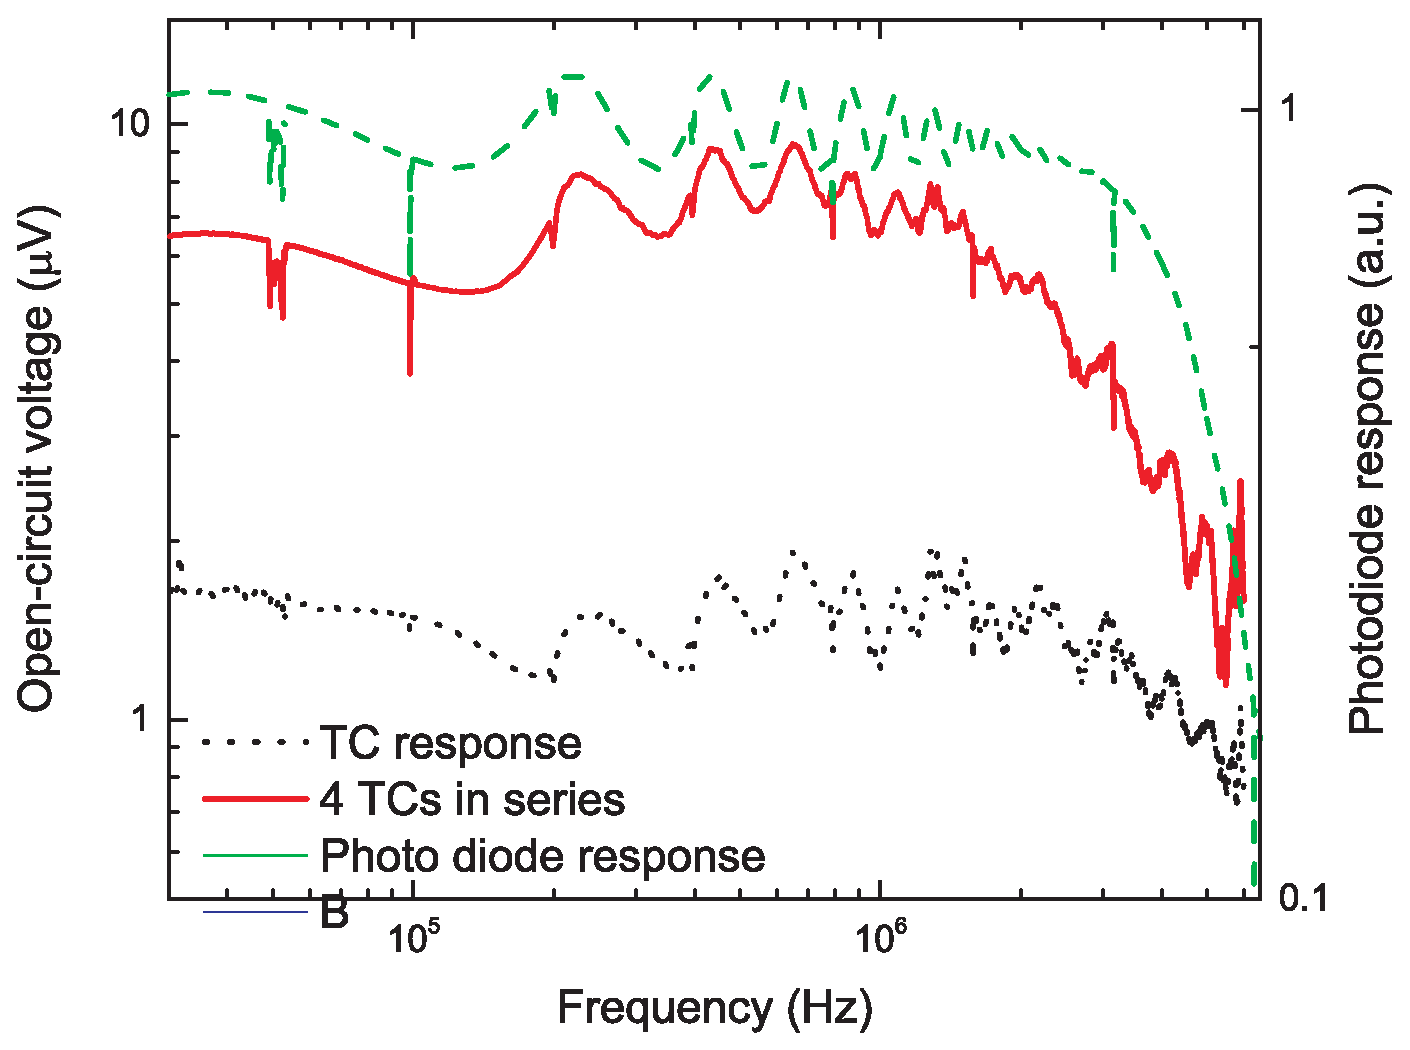
\includegraphics[width=1.0\columnwidth,clip]{figures/Fig12n}}
\caption{Frequency-dependent response of the NTCs and a four-NTC-long thermopile. The reference measurement shows frequency-dependent intensity of the laser beam caused by the AOM.}
\label{fig4}
\end{figure}
%
From the figure we can determine that the -3 dB level of the measured signal is about 3.9 MHz. However, there is no physical reason to believe that the attenuation of the measured NTC signal is due to the thermal time constant of the NTC, rather it is caused by: 1) parasitic low-pass filtering, 2) frequency-dependent intensity of the modulated laser beam.

First, the resistance of the lead lines of the NTC (8 k$\Omega$) along with the cable capacitances form a low-pass filter, which limits the bandwidth of the measurements. This effect is evident form the different -3dB levels of the single NTC (3.9 MHz) and the thermopile (3.5 MHz), which has about four times larger resistance and cable capacitance.

Second, the intensity of the modulated laser beam is frequency dependent as shown in Fig.~\ref{fig4} by the output beam intensity of the AOM measured by a photo diode (PD). Therefore, the incident power on the NTC as a function of frequency is not uniform, which results in an attenuation of the measured signal.

Figure~\ref{fig4} also shows that by comparing the NTC response to the PD response that the fluctuation in the measured thermal response is not the property of the NTC, rather a frequency-dependent intensity fluctuation of the laser beam introduced to the system by the AOM.

%
%-----------------------------------------------------------------------------------------------------------------------------------------------------------------------
%
\section{Conclusion and Outlook}
%
%-----------------------------------------------------------------------------------------------------------------------------------------------------------------------
%
In this work we describe the design, fabrication, and theoretical and experimental investigation of single-metal ACNTCs. ACNTCs are excellently suited as polarization-sensitive detectors and mixers for the long-wavelength far-infrared range around 30 THz. The theoretical fundamentals of the geometry-dependent Seebeck effect facilitating single-metal ACNTCs have been discussed.  In thin films, the influence of surface electron scattering on the mean free path of the electrons yields a geometry dependence of the Seebeck effect, and makes SMTCs possible. We have given the experimental evidence for single-metal ACNTCs. The theoretical analysis of the thermal dynamics of NTCs has shown that detector low-frequency bandwidths and mixer intermediate-frequency beyond 100~GHz could be expected. This makes TCs presently the fastest THz detectors, suitable for broadband detector and heterodyne receiver applications. The combination with state of the art coherent terahertz sources, such as quantum cascade laser structures for room temperature terahertz frequency conversion~\cite{vijayraghavan2013broadly, jirauschek2013monte,lu2014continuous}, will pave the way for many innovative applications.

We experimentally demonstrated that ACNTCs are capable to detect and rectify long-wave infrared radiation at 10.6~$\mu$m wavelength. We also demonstrated that such NTCs are able to follow thermal oscillations in the MHz range, however, the bandwidth limitations of our experimental setup does not allow the determination of the cut-off frequency of these devices. 

Although our experimental investigations proved that NTCs exhibit detection bandwidths at least in the MHz range and consequently will be applicable for many sensing and communications applications, our theoretical investigations have shown that intermediate frequency bandwidths in mixer applications and low-frequency bandwidths in detector applications, both in the order of 100~GHz will be feasible. This will open the door for novel future applications in the THz bands. Future detector and mixer experiments with ACNTCs excited by two-frequency far-infrared signals should will push forward the experimental validation of the broadband detector and mixer properties of ACNTCs.

%
%---------------------------------------------------------------------------------------------------------------------------------------------------------------------------------
%
\section*{Acknowledgement}
%
%---------------------------------------------------------------------------------------------------------------------------------------------------------------------------------
%
Christian Jirauschek thanks the Deutsche Forschungsgemeinschaft for funding under the project DFG JI 115/4-1.
Gergo P.~Szakmany gratefully acknowledges financial support from the Notre Dame Joseph F. Trustey Fund for Postdoctoral Scholars.

%
%----------------------------------------------------------------------------------------------------------------------------------------------
%%
\bibliographystyle{IEEEtran}
\bibliography{MTT_thermocouple}

%
%
\begin{IEEEbiography}
[{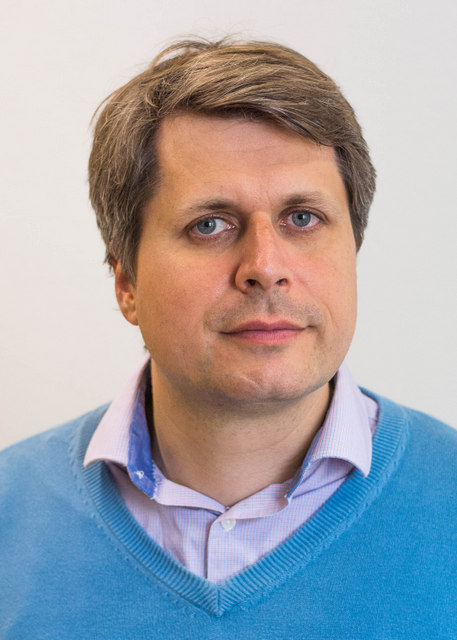
\includegraphics[width=1in,height=1.25in,clip,keepaspectratio]{figures/JohannesRusser}}]{Johannes A. Russer} received his Dipl.-Ing. (M.S.E.E.) degree in electrical engineering and information technology from the Universit\"at Karlsruhe, Germany, in 2003. In 2004, he joined the University of Illinois at Urbana-Champaign as a research assistant where he received his Ph.D.E.E. degree in 2010. From 2007 to 2010, he has been working for Qualcomm Inc. as
an intern. In 2008, he received a Best Student Paper Award at the IEEE International Microwave Symposium. Since 2010, he is a Postdoctoral Research Fellow at the Institute of Nanoelectronics of the Technische Universit\"at M\"unchen (TUM), Germany. In 2015, Johannes Russer received the best paper award from the ITG (German Society for Information Technology). He is a member of VDE, IEEE, and of the Eta Kappa Nu honor society.
\end{IEEEbiography}
%
%
\begin{IEEEbiography}
   [{
\includegraphics[width=1in,height=1.25in,clip,keepaspectratio]{figures/Christian_Jirauschek}}]{Christian Jirauschek} received his Dipl.-Ing. and doctoral degrees in electrical engineering from Universit\"at Karlsruhe (TH), Germany, in 2000 and 2004, respectively. From 2002 to 2005, he worked at the Massachusetts Institute of Technology (MIT). He then joined the Institute of Nanoelectronics at Technische Universit\"at M\"unchen (TUM), Germany, where since 2007 he headed an independent junior research group within the Emmy Noether program of the Deutsche Forschungsgemeinschaft (DFG). In 2014, he received a Heisenberg professorship grant from the DFG. His research interests include modeling in the areas of photonics and nanoelectronics.
\end{IEEEbiography}
 %
 %
\begin{IEEEbiography}
[{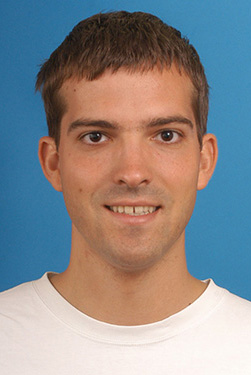
\includegraphics[width=1in,height=1.25in,clip,keepaspectratio]{figures/Gergo_Szakmany}}]
{Gergo P. Szakmany} received his diploma in electrical and computer engineering from the Pazmany Peter Catholic University, Budapest, Hungary in 2007. He received his MS and PhD degrees in electrical engineering from the University of Notre Dame, Notre Dame, IN in 2011 and 2013, respectively. He is continuing his research at the University of Notre Dame on antenna-coupled infrared detectors as a Postdoctoral Research Associate. His research interests focuses on submicron device fabrication and characterization.
\end{IEEEbiography}
%
%
\begin{IEEEbiography} 
[{\includegraphics[width=1in,height=1.25in,clip,keepaspectratio]{figures/Mark_Schmidt}}]{Mark Schmidt} received his B.Sc. degree from the Technische Universit\"at M\"unchen (TUM), Germany, in 2014, where he specialized on high frequency engineering. He is currently pursuing a M. Sc. degree at TUM, and is working at the Institute of Nanoelectronics on the modeling of infrared-range thermocouple detectors. His research interests include theory, design, and applications in the areas of photonics, radio-frequency engineering and energy harvesting.
\end{IEEEbiography}
%
%
\begin{IEEEbiography}
   [{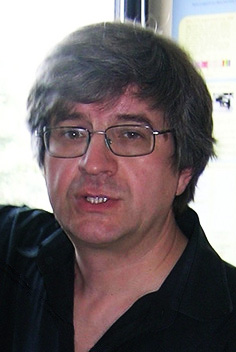
\includegraphics[width=1in,height=1.25in,clip,keepaspectratio]{figures/Alexei_Orlov}}]{Alexei O. Orlov} currently is a Research Professor at the University of Notre Dame. He received his M.S. degree in Physics from the Moscow State University in 1983. From 1983 to 1993 he worked at the Institute of Radio Engineering and Electronics of the Russian Academy of Sciences, Moscow. During this time he conducted research on mesoscopic and quantum ballistic effects in electron transport of GaAs field-effect transistors.
   
He received his Ph.D. from the same Institute in 1990. He was a visiting fellow at the University of Exeter, UK in 1993, and joined the Department of Electrical Engineering at the University of Notre Dame, IN, in 1994. His research interests include experimental studies of mesoscopic, single-electron and molecular electronic devices and sensors, nanomagnetics and quantum-dot cellular automata. Alexei Orlov has authored or co-authored more than 150 journal publications.
\end{IEEEbiography}
% 
\begin{IEEEbiography}
   [{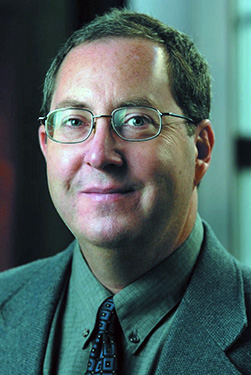
\includegraphics[width=1in,height=1.25in,clip,keepaspectratio]{figures/Gary_Bernstein}}]{Gary H. Bernstein} received his BSEE from the University of Connecticut, Storrs, with honors, in 1979 and MSEE from Purdue University, W. Lafayette, Indiana in 1981. During the summers of 1979 and '80, he was a graduate assistant at Los Alamos National Laboratory, and in the summer of 1983 interned at the Motorola Semiconductor Research and Development Laboratory, Phoenix, Arizona. He received his Ph.D. in Electrical Engineering from Arizona State University, Tempe, in 1987, after which he spent a year there as a postdoctoral fellow. He joined the Department of Electrical Engineering at the University of Notre Dame, Notre Dame, Indiana, in 1988 as an assistant professor, and was the founding Director of the Notre Dame Nanoelectronics Facility (NDNF) from 1989 to 1998. Dr. Bernstein received an NSF White House Presidential Faculty Fellowship in 1992, was promoted to rank of Professor in 1998, and served as the Associate Chairman of his Department from 1999 to 2006. Bernstein was named a Frank M. Freimann Professor of Electrical Engineering in 2010. He has authored or co-authored more than 200 publications in the areas of electron beam lithography, nanomagnetics, quantum electronics, high-speed integrated circuits, electromigration, MEMS, and electronics packaging.
\end{IEEEbiography}
%
%
\begin{IEEEbiography} 
[{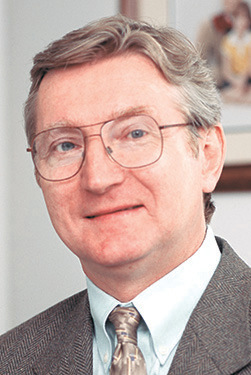
\includegraphics[width=1in,height=1.25in,clip,keepaspectratio]{figures/Wolfgang_Porod}}]{Wolfgang Porod} currently is Frank M. Freimann Professor of Electrical Engineering at the University of Notre Dame. He received his Diplom (M.S.) and Ph.D. degrees from the University of Graz, Austria, in 1979 and 1981, respectively. After appointments as a postdoctoral fellow at Colorado State University and as a senior research analyst at Arizona State University, he joined the University of Notre Dame in 1986 as an Associate Professor. He now also serves as the Director of Notre Dame's Center for Nano Science and Technology. 

His research interests are in the area of nanoelectronics, with an emphasis on new circuit concepts for novel devices. He has authored some 300 publications and presentations. He has served as the Vice President for Publications for the IEEE Nanotechnology Council (2002-2003), and he was appointed an Associate Editor for the IEEE Transactions on Nanotechnology (2001-2005). He has been active on several committees, in organizing special sessions and tutorials, and as a speaker in IEEE Distinguished Lecturer Programs. He is a Fellow of the IEEE.
\end{IEEEbiography}
%%
\begin{IEEEbiography}
[{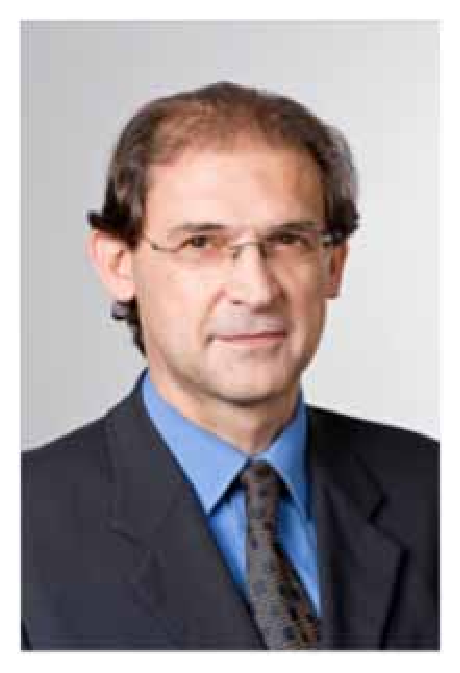
\includegraphics[width=1in,height=1.25in,clip,keepaspectratio]{figures/Paolo_Lugli}}]
{Paolo Lugli} graduated in Physics at the University of Modena, Italy, in 1979. In 1981 he joined Colorado State University, Fort Collins, CO, where he received his Master of Science in 1982 and his Ph.D. in 1985, both in Electrical Engineering. In 1985 he joined the Physics Department of the University of Modena as Research Associate. From 1988 to 1993 he was Associate Professor of ``Solid State Physics'' at the ``Engineering Faculty'' of the 2nd University of Rome ``Tor Vergata''. In 1993 he was appointed as Full Professor of ``Optoelectronics'' at the same University. In 2002 he joined the Technical University of Munich where he was appointed head of the newly created Institute for Nanoelectronics.

His current research interests involve, beside nanoimprint lithography, the modeling, fabrication and characterization of organic devices for electronics and optoelectronics applications, the design of circuits and architectures for nanostructures and nanodevices, the numerical simulation of microwave semiconductor devices, and the theoretical study of transport processes in nanostructures. 
He is author of more than 350 scientific papers and co-author of the books ``The Monte Carlo Modelling for Semiconductor Device Simulations'' (Springer, 1989) and ``High Speed Optical Communications'' (Kluver Academic, 1999). In 2004, he served as General Chairman of the IEEE International Conference on Nanotechnology held in Munich. He is IEEE Fellow and member of the German National Academy of Science and Engineering (acatech).
\end{IEEEbiography}
%
%
\begin{IEEEbiography}
[{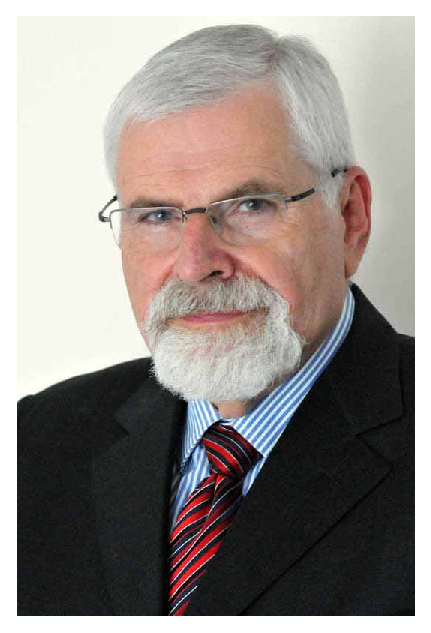
\includegraphics[width=1in,height=1.25in,clip,keepaspectratio]{figures/Peter_Russer}}]
{Peter Russer} received the Dipl.-Ing. (M.S.E.E.) degree in 1967 and the Dr. techn.  (Ph.D.E.E.) degrees in 1967 and 1971, respectively, both from the Vienna University of Technology, Austria. In 1971 he joined the Research Institute of AEG-Telefunken in Ulm, Germany. From 1981 to 2008 Peter Russer has been Professor and head of the Institute for High Frequency Engineering at the Technische Universit\"at M\"unchen (TUM), Germany. From October 1992 to March 1995 he also has been Director of the Ferdinand-Braun-Institut f\"ur H\"ochstfrequenztechnik, Berlin. From 1997 to 1999 he has been Dean of the Department of Electrical Engineering and Information Technology of the TUM. 

The current research interests of Peter Russer include electromagnetic fields, numerical electromagnetics, metamaterials, integrated microwave and millimeter-wave circuits, statistical noise analysis, electromagnetic compatibility, and  quantum nanoelectronics.
He has published  more than 800 scientific papers and among five books the book ``Electromagnetics, Microwave Circuit and Antenna Design for Communications Engineering'' (Boston 2006). In 1994 he was elected Fellow of  IEEE and in 2013 he became Life Fellow of  IEEE. In 2006 he was elected member of acatech. In 2006 he received the Distinguished Educator Award and in 2012 the Microwave Pioneer Award, both of the IEEE MTT Society, and in 2009 the Distinguished Service Award from the European Microwave Association. In 2007 he received an honorary Doctor degree from the Moscow University of Aerospace Technologies. In 2010 he was awarded the Golden Ring of Distinction of the German Association for Electrical, Electronic and Information Technologies (VDE). 
\end{IEEEbiography}
%
\end{document}















